\documentclass[a4paper,10pt]{report}
\usepackage[T1]{fontenc}
\usepackage[table]{xcolor}
\usepackage{titlesec}
\usepackage{graphicx}
\usepackage[inkscapepath=../assets/svg]{svg}
\usepackage{amsmath}
\usepackage{amsthm}
\usepackage{mathtools}
\usepackage{fancyvrb}
\usepackage[english]{babel}
\usepackage{csquotes}
\usepackage{hyperref}
\hypersetup{
   colorlinks=true,
   linkcolor=blue,
   urlcolor=cyan
}
\usepackage{tikz}
\usepackage{amssymb}
\usepackage[sc]{mathpazo}
\linespread{1.05}
\usepackage{microtype}
\usepackage{breqn}
\usepackage{caption}
\usepackage{subcaption}
\usepackage[
   backend=bibtex,%
   bibencoding=utf8,%
   language=english,%
   style=numeric-comp,%
   sorting=nyt,%
   maxbibnames=10,%
   natbib=true%
]{biblatex}
\addbibresource{references.bib}
\usepackage{siunitx}
\usepackage{booktabs}
\usepackage{longtable}
\usepackage{geometry}
\graphicspath{ {../assets/img/} }

\newgeometry{hmargin={30mm,30mm}}

% Set TOC depth and sections numbering
\setcounter{tocdepth}{3}
\setcounter{secnumdepth}{3}

% Remove chapters head and reduce spacing
\titleformat{\chapter}[hang]{\Large\bfseries}{\thechapter \hspace{2ex}}{0pt}{\Large}
\titlespacing{\chapter}{0cm}{0cm}{0.5cm}
\usepackage[parfill]{parskip}

% Make quotes italic
\renewcommand{\mkbegdispquote}[2]{\itshape}

% Change texttt line breaks
\renewcommand{\texttt}[1]{%
  \begingroup
  \ttfamily
  \begingroup\lccode`~=`.\lowercase{\endgroup\def~}{.\discretionary{}{}{}}%
  \catcode`/=\active\catcode`[=\active\catcode`.=\active
  \scantokens{#1\noexpand}%
  \endgroup
}


\begin{document}
\frenchspacing

% First page
\title{
	{{\large{\textsc{Alma Mater Studiorum $\cdot$ University of Bologna}}}}
	\rule{\textwidth}{0.4pt}\vspace{3mm}
	\textbf{Question answering on the SQuAD dataset}
	\begin{figure}[!htb]
		\centering
		
\includegraphics[width = 100pt]{squad-logo}
	\end{figure} \\
	NLP course final project
}

\author{Leonardo Calbi (\href{mailto:leonardo.calbi@studio.unibo.it}{leonardo.calbi@studio.unibo.it}) \\ Lorenzo Cellini (\href{mailto:lorenzo.cellini3@studio.unibo.it}{lorenzo.cellini3@studio.unibo.it}) \\ Alessio Falai (\href{mailto:alessio.falai@studio.unibo.it}{alessio.falai@studio.unibo.it})}
\date{\today}
\maketitle
\newpage
\tableofcontents
\setcounter{tocdepth}{1}
%\listoffigures
%\listoftables
\newpage


\chapter{Summary}\label{chap:introduction}

The tasks of machine comprehension (MC) and question answering (QA) have gained significant popularity over the past few years within the natural language processing and computer vision communities. Systems trained end-to-end now achieve great results on a variety of tasks in the text and image domains.

In this work we address a question answering problem and, in particular, the Stanford Question Answer Dataset (SQuAD) problem: given a large collection of Wikipedia articles with associated questions, the goal is to identify the span of characters that contains the answer to the question.

This project focuses on the SQuAD v1.1 dataset, that contains more than 100,000 question-answer pairs on more than 500 articles. Here each question has at least one associated answer, whereas in the SQuAD v2.0 dataset there are also questions with no answers at all.

In this work we implement and compare three different models: a naïve LSTM encoder-decoder that will act as our baseline, the Bi-Directional Attention Flow (BIDAF) network (CITAZIONE) and a model that wraps a pretrained Bidirectional Encoder Representations from Transformers (BERT), as language model, coupled with a custom output layer on top of it.

Our experimental evaluations show that our models achieve …………………………………………….

\chapter{Background}\label{chap:background}

As already described above, the question answering task is based on the idea of identifying one possible answer to the given question as a subset of the given context. 

Since the input data is of textual form and the latest models for the task are all based on neural architectures, there is the need to encode such text into a numeric representation. As of today, there are two main approaches to embed words in numerical format: sparse embeddings, like TF-IDF \cite{tf-idf} and PPMI \cite{ppmi}, and the modern dense embeddings, such as Word2Vec \cite{word2vec} and GloVe \cite{glove}. In the latter case, embeddings for each word in the input vocabulary are usually computed with shallow encoders. 

These emebddings are then used as inputs for models specialized in processing sequential inputs. Nowadays, such models are mostly based on the Transformer architecture \cite{transformers}, which has the attention mechanism at its core. Instead, before this revolution, NLP competition's leaderboards were mostly populated by models based on recurrent and convolutional modules.

The most influential recurrent networks are LSTMs \cite{lstm} and GRUs \cite{gru}. They are both based on processing sequential inputs and they keep an evolving series of hidden states, such that the output $h_t^{(0)}$ is a function of $h_{t-1}^{(0)}$ and the input $x_t$ at position $t$. Recurrent layers can also be stacked to increase the capacity of the network: in that case, $h_t^{(0)}$ would act as an input to $h_t^{(1)}$, i.e. the first hidden state of the next depth-wise layer, and the same goes for the successive layers, as shown in figure \ref{fig:recurrent}.

\begin{figure}[h]
    \center
    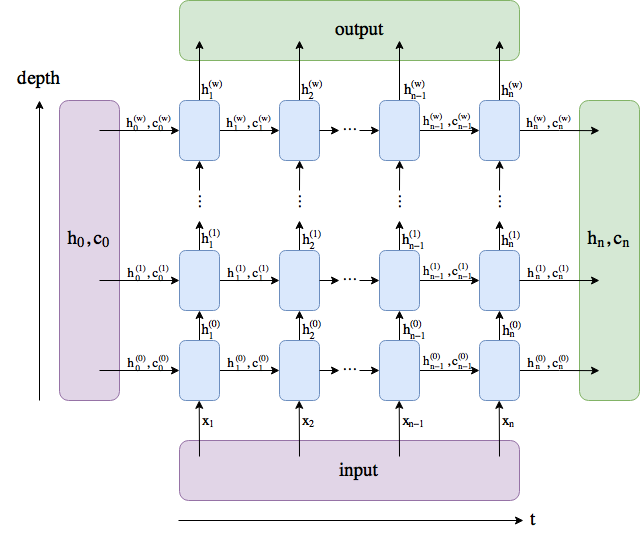
\includegraphics[width=0.65\linewidth]{recurrent}
    \caption{Recurrent module (image courtesy of \cite{recurrent-img})}
    \label{fig:recurrent}
\end{figure}

Since RNNs are not well suited for keeping track of long-term dependencies, some refined 
modules were invented just for that. One example of such improvement is bi-directionality: the input is processed in two ways, from left to right (the "forward" pass) and from right to left (the "backward" pass); then, outputs of the two computations are merged together (usually by concatenating them over their last dimension). The intuition behind bi-directional RNNs is that they tend to understand the overall context better than their uni-directional counterparts, since they are able to aggregate information from the "past" and from the "future".

About Transformers, at a high-level, they comprise a stack of encoder-decoder modules, where each encoder features a multi-head attention block (to focus on different subsets of the input sequence when encoding one specific token) and a point-wise fully-connected layer, while each decoder features the same architecture as the encoder, but with an additional multi-head attention block in the middle (that helps the decoder focus on relevant parts of the input sequence).

The multi-head attention modules in the Transformer architecture are the ones responsible for gathering information from other tokens in the input sequence, thus resembling the task of hidden states in RNNs (i.e. incorporate the representation of previous inputs with the currently processed one).

\begin{figure}[h]
    \center
    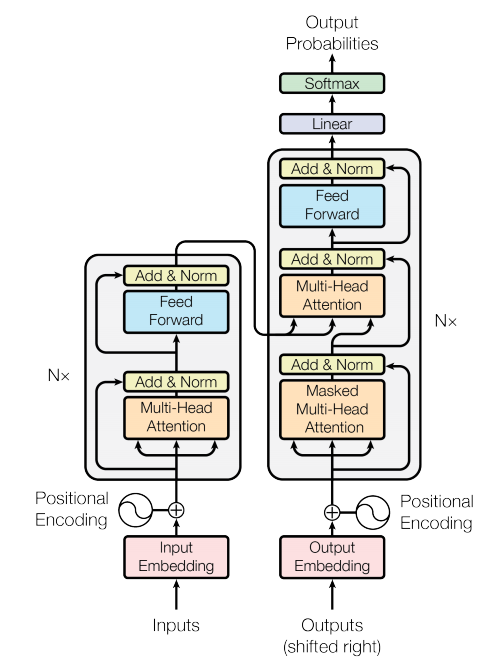
\includegraphics[width=0.45\linewidth]{transformers}
    \caption{Transformers (image taken from \cite{transformers})}
    \label{fig:transformers}
\end{figure}

While Transformers may always seem the way to go, since they throw away all the computational burden of training recurrent modules (which are sequential in nature and, thus, scarcely parallelizable), they also suffer from limitations due to the quadratic complexity of attention and the inherent maximum number of input tokens (which is implicitly linked to architecture choices themselves).


\chapter{System description}\label{chap:system-description}

In this work we implement three distinct models: a naïve LSTM encoder-decoder that will act as our baseline, the Bi-Directional Attention Flow (BIDAF) network (CITAZIONE) and a model that wraps a pretrained Bidirectional Encoder Representations from Transformers (BERT), as language model, coupled with a custom output layer on top of it.

Each model is trained on the SQuAD v1.1 training set and evaluated on the SQuAD v1.1 dev set, available on the github repository of the SQuAD project (link).

The models’ evaluation is carried out on the same preprocessed data: indeed, we defined a preprocessing pipeline, applied it to the training and dev set once and the resulting dataset is fed to each model. (CONTROLLARE QUI – mi pare che per bert abbiamo tokenizzato diversamente)

In order to perform an effective models’ comparison, each model shares the same input and output layer: what changes is the language model (embedding + attention layers) and the modelling layer.

The following is a detailed description of the models.

\section{Baseline}\label{sec:baseline}

….

\section{BiDAF}\label{sec:bidaf}

Sintesi tra paper bidaf e medium

\section{BERT}\label{sec:bert}

….

\chapter{Experimental setup and results}\label{chap:experiments}

\chapter{Analysis of results}\label{chap:analysis-results}

\chapter{Discussion}\label{chap:discussion}

\printbibliography

\end{document}
